\documentclass[11pt]{article}

\usepackage{exsheets}
\usepackage[paper=a4paper, headheight=110pt,showframe=false, 
            layoutvoffset=2em,
            bottom=2cm, top=3.5cm]{geometry}

\usepackage[spanish]{babel}
\usepackage[babel]{microtype}
\usepackage{lipsum}
\usepackage{unicode-math}
% Fonts can be customized here.
\defaultfontfeatures{Mapping=tex-text}
\setmainfont [Ligatures={Common}]{Linux Libertine O}
\setmonofont[Scale=0.9]{Linux Libertine Mono O}
%\usepackage[svgnames]{xcolor} % Gestión de colores
\usepackage{hyperref}
\hypersetup{
  colorlinks=true, linktocpage=true, pdfstartpage=3, pdfstartview=FitV,%
  breaklinks=true, pageanchor=true,%
  pdfpagemode=UseNone, %
  plainpages=false, bookmarksnumbered, bookmarksopen=true, bookmarksopenlevel=1,%
  hypertexnames=true, pdfhighlight=/O,%nesting=true,%frenchlinks,%
  urlcolor=Maroon, linkcolor=RoyalBlue, citecolor=Blue, %pagecolor=RoyalBlue,%
  pdftitle={},%
  pdfauthor={\textcopyright\ C. Manuel Carlevaro},%
  pdfsubject={},%
  pdfkeywords={},%
  pdfcreator={XeLaTeX},%
  pdfproducer={XeLaTeX}%
}

\usepackage{hyperref}
\usepackage{fontawesome, gensymb}
\usepackage{graphicx}
\setlength{\parindent}{3em}
\setlength{\parskip}{1em} 
\usepackage[shortlabels]{enumitem}

%\NewDocumentCommand{\evalat}{sO{\big}mm}{%
  %\IfBooleanTF{#1}
   %{\mleft. #3 \mright|_{#4}}
   %{#3#2|_{#4}}%
%}


\title{Cálculo avanzado}
\author{Dpto. de Ingenería Mecánica}
\date{Clase 2: números complejos}


\begin{document}

\begin{center}
\framebox[1.0\textwidth][c]{
\huge{\textsc{Cálculo Avanzado}} 
}
\end{center} 

\begin{center}
\vspace{\baselineskip}
\Large{\textsc{Departamento de Ingenería Mecánica}} \\
\textsc{Facultad Regional La Plata} \\
\textsc{Universidad Tecnológica Nacional}
\end{center}

% \vspace{1em}
%%%% Formato de problemas:
% Cada problema tiene el formato:
% \begin{question} % Referencia del problema
%   \begin{enumerate}[a)] % En caso que haya ítems del problema
%   \end{enumerate}
% \end{question}
%%%%

\begin{center}
\begin{tabular}{r l}
    \textbf{Práctica:} & 2 \\
 \textbf{Tema:} & Introducción a la variable compleja. \\
 \textbf{Profesor Titular:} & Manuel Carlevaro \\
 \textbf{Jefe de Trabajos Prácticos:} & Diego Amiconi \\
 \textbf{Ayudante de Primera:} & Lucas Basiuk 
\end{tabular}\end{center}

\vspace{1em}

\begin{question} % H. Gross - 1.8.1(L) pg 3.
    \begin{enumerate}[a)]
        \item Calcular:
        \[ \int_0^{2i} z dz \]
    \item Calcular:
        \[ \int_0^{2 i} \bar{z} dz \]
\end{enumerate}
primero a lo largo del segmento de línea $C_1$ que une $0$ con $2i$, y luego a lo largo de la curva $C_2$, donde $C_2$ es la mitad derecha del círculo centrado en $i$ con radio $1$.
\end{question}

\begin{question} % H. Gross - 1.8.2 pg 3.
Explicar por qué la integral:
\[ \int_1^i 2 e^{2z} \, dz \]
no es ambigua, y encontrar el valor de esta integral.
\end{question}

\begin{question}  % H. Gross - 1.8.3 pg 3.
    Calcular:
    \[ \int_1^i \bar{z}^2 \, dz \]
    a lo largo de las siguientes curvas $C$:
    \begin{enumerate}[a)]
        \item $C$ es el segmento de línea que une $1$ con $i$.
        \item $C = \{z : z = e^{i \theta}, \; 0 \leq \theta \leq \dfrac{\pi}{2}\} $, es decir, $C$ es el primer cuadrante del círculo $|z| = 1$.
    \end{enumerate}
\end{question}

%% \TODO : ver cómo insertar una imagen en un problema.
%\begin{wrapfigure}[6]{r}[3em]{0.25\textwidth}
    %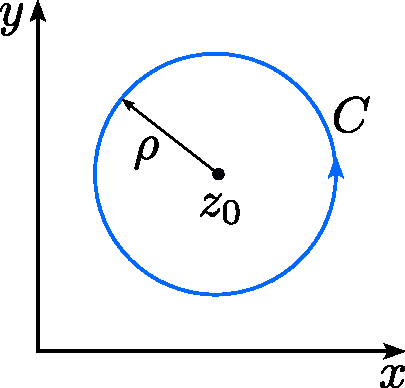
\includegraphics[width=0.25\textwidth]{figs/fig-10.pdf}
    %\caption{Ejercicio 4.}
%\end{wrapfigure}
\begin{question}  % Kreyszig example 6, pg 649
Sea $f(z) = (z - z_0)^m$, donde $m$ es un entero y $z_0$ una constante. Integrar la función sobre una trayectoria circular $C$ de radio $\rho$ con centro en $z_0$ en sentido antihorario. 
\end{question}


\begin{question}% H. Gross - 1.7.1(L) pg 3.
    Suponga que $\lim_{n \rightarrow \infty} a_n = L_1$ y $\lim_{n \rightarrow \infty} a_n = L_2$. Probar que $L_1 = L_2$.
\end{question}

\begin{question}  % H. Gross - 1.7.2(L) pg 3
Sea $f(z)$ definida por
\[ f(z) = 1 - 2 z + 3 z^2 -4 z^3 + \cdots = \sum_{n=0}^{\infty} (-1)^n (n + 1) z^n \]
\begin{enumerate}[a)]
    \item Encuentre el radio de convergencia de $f$.
    \item Calcule $f(\tfrac{i}{12})$ con una precisión dada por un disco de radio $0.001$.
    \item Calcule $f'(\tfrac{i}{12})$ con una precisión de un dígito decimal.
\end{enumerate}
\end{question}

\end{document}
